\section{Стабилизация неустойчивых стационарных решений уравнения Бюргерса}
\vspace{1em}

Рассмотрим вязкое уравнение Бюргерса:

\begin{equation}\label{burger}
  u_t = u_{xx} - u_x u, \quad 0 < x < 1, \quad t > 0
\end{equation}

с начальным и граничными условиями:

\begin{gather}\label{cond}
  u(0, t) = w_1(t), \\*
  u(1, t) = w_2(t), \\*
  u(x, 0) = u_{0}(x) \in L^2(0, 1). \nonumber
\end{gather}

\begin{remark}
Уравнение Бюргерса обычно изучается в форме $u_t = \epsilon u_{xx} - u_xu$, в этой работе рассматривается система с $\epsilon = 1$. Все результаты могут быть получены для любого $\epsilon \ne 1$
\end{remark}

Рассмотрим семейство стационарных решений shock-like

\begin{equation}\label{shock_like}
  U(x) = -2\sigma\tanh{(\sigma(x - \frac{1}{2}))},
\end{equation}

где параметр $\sigma \ge 0$.

\begin{figure}[H]
  \centering
  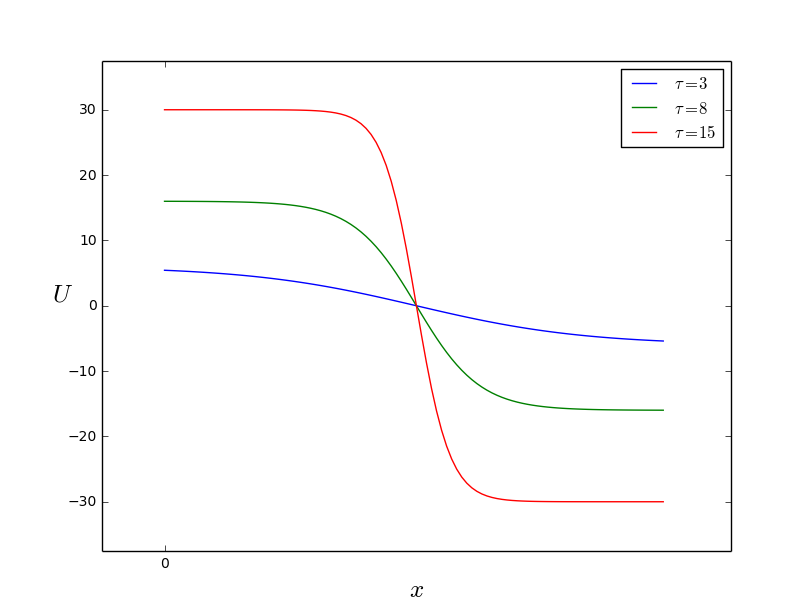
\includegraphics[width=4in]{fig1}
  \caption{Три примера $U(x)$ при разных $\sigma$}
\end{figure}

В качестве \eqref{cond} возмем

\begin{gather}\label{cond2}
  w_1(t) = U(0) \\*
  w_2(t) = U(1)
\end{gather}

Введем новое обозначение

\begin{equation}
  \hat{u}(x, t) = u(x, t) - U(x)
\end{equation}

Тогда, уравнение \eqref{burger} перепишется через новую переменную $\hat{u}$

\begin{equation}\label{fluct}
    \hat{u}_t = \hat{u}_{xx} - U(x)\hat{u}_x - U'(x)\hat{u} - \hat{u}_x\hat{u}
\end{equation}

Начальные и граничные условия перепишутся в виде

\begin{gather}\label{fluct_cond}
  \hat{u}(0, t) = 0 \\*
  \hat{u}(1, t) = 0 \\*
  \hat{u}(x, 0) = u_{0}(x) - U(x) \in L^2(0, 1). \nonumber
\end{gather}

\subsection{Неустойчивость shock-like стационарного решения}

Для изучения устойчивости системы \eqref{fluct} - \eqref{fluct_cond}, мы линеаризуем её

\begin{gather}\label{linearized}
  \theta_t = \theta_{xx} + 2 \sigma (\tanh(\sigma(x - \frac{1}{2}))\theta)_x \\*
  \theta(0, t) = \theta(1, t) = 0,
\end{gather}

где $\theta(x, t)$ линеаризация $\hat{u}$. \eqref{linearized} - уравнение конвенкции-диффузии-реакции. Для простоты изучения устойчивости, мы избавимся от конвекционого члена используя преобразование $\zeta(x, t) = G(x)\theta(x, t)$, где 

\begin{equation}
  G(x) = \frac{\cosh(\sigma(x - \frac{1}{2}))}{\cosh(\frac{\sigma}{2})}
\end{equation} 

Имеем 

\begin{gather} \label{transf_linear}
  \zeta_t = \zeta_{xx} + \sigma^2 \left( \frac{2}{\cosh^2(\sigma(x - \frac{1}{2}))} - 1 \right) \zeta \\* 
  \zeta(0) = \zeta(1) = 0 
\end{gather}

Для $\sigma = 0$ система нейтрально устойчива. Для $\sigma > 0$,  реакционный член в \eqref{transf_linear} также является неустойчивым в окрестности $x = \frac{1}{2}$ (Рис 2.)


\begin{figure}[H]
  \centering
  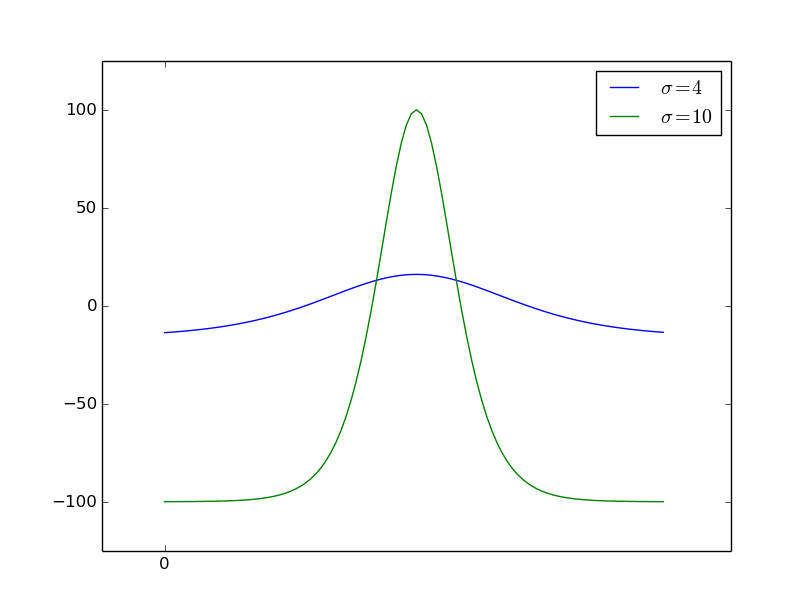
\includegraphics[width=4in]{fig2}
  \caption{Значение реакционного члена в \eqref{transf_linear}}
\end{figure}





